\documentclass[aspectratio=169,11pt]{beamer}

% ======================
% STYLE
% ======================
\usepackage[utf8]{inputenc}
\usepackage[T1]{fontenc}
\usepackage{lmodern}
\usepackage{amsmath,amssymb,bm}
\usepackage{appendixnumberbeamer}
\usepackage{tikz}
\usetikzlibrary{positioning,decorations.pathmorphing,decorations.pathreplacing,arrows.meta}
\graphicspath{{../thesis_latex/figures/}}

\usetheme{default}
\usefonttheme{professionalfonts}
\definecolor{tblue}{HTML}{0072B2}
\definecolor{torange}{HTML}{D55E00}
\definecolor{tgrey}{HTML}{555555}
\setbeamercolor{structure}{fg=tblue}
\setbeamercolor{frametitle}{fg=black}
\setbeamerfont{frametitle}{size=\Large,series=\bfseries}
\setbeamertemplate{navigation symbols}{}
\setbeamertemplate{itemize items}{\color{tblue}$\bullet$}
\setbeamertemplate{footline}{%
  \hfill{\scriptsize\color{tgrey}\insertframenumber\,/\,\inserttotalframenumber}\hspace{1.2em}\vspace{0.8em}}

\title{Dissipation Assisted Matrix Product Factorization\\ for Quantum Heat Engines}
\subtitle{Vibronic enhancement beyond a single mode}
\author{Tommaso Galletti}
\institute{Università degli Studi di Milano -- Dipartimento di Fisica\\[4pt]
  {\small Supervisor: Prof.~Dario Tamascelli \quad Co-supervisor: Prof.~Claudia Benedetti}}
\date{19 November 2026}

\begin{document}

% ---------------------------------------------------------------- 1
\begin{frame}[plain]
  \titlepage
\end{frame}

% ---------------------------------------------------------------- 2
\begin{frame}{Motivation}
  \begin{itemize}\setlength\itemsep{0.9em}
    \item Light-harvesting complexes transfer the absorbed energy to a reaction center with high efficiency, at room temperature
    \item Two-dimensional spectroscopy: long-lived oscillations, attributed to underdamped vibrations close to resonance with the excitonic gaps \\
      {\small\color{tgrey} Engel \textit{et al.} 2007; Christensson \textit{et al.} 2012; Chin \textit{et al.} 2013}
    \item Killoran, Huelga and Plenio (2015): the light harvester as a quantum heat engine, in which a resonant vibrational mode increases the output power
    \item In this thesis: a larger part of the vibrational environment is described explicitly, with more modes and modes off resonance
  \end{itemize}
\end{frame}

% ---------------------------------------------------------------- 3
\begin{frame}{Electronic model: the four-level quantum heat engine}
  \begin{columns}[c]
    \begin{column}{0.50\textwidth}
      \centering
      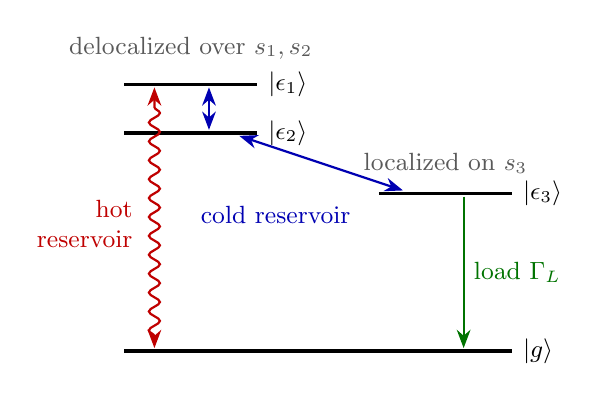
\begin{tikzpicture}[>=Stealth, lev/.style={very thick}, every node/.style={font=\small}, scale=0.77]
        \draw[lev] (0,0) -- (6.4,0) node[right] {$|g\rangle$};
        \draw[lev] (0,4.4) -- (2.2,4.4) node[right] {$|\epsilon_1\rangle$};
        \draw[lev] (0,3.6) -- (2.2,3.6) node[right] {$|\epsilon_2\rangle$};
        \draw[lev] (4.2,2.6) -- (6.4,2.6) node[right] {$|\epsilon_3\rangle$};
        \draw[<->, thick, red!75!black, decorate, decoration={snake, amplitude=0.7mm, segment length=2.4mm, pre length=1.5mm, post length=1.5mm}] (0.5,0.05) -- (0.5,4.35);
        \node[red!75!black, align=right, anchor=east] at (0.3,2.1) {hot\\ reservoir};
        \draw[<->, thick, blue!70!black] (1.4,4.35) -- (1.4,3.65);
        \draw[<->, thick, blue!70!black] (1.9,3.55) -- (4.6,2.65);
        \node[blue!70!black, anchor=north] at (2.5,2.55) {cold reservoir};
        \draw[->, thick, green!45!black] (5.6,2.55) -- (5.6,0.05) node[midway, right] {load $\Gamma_L$};
        \node[gray!70!black] at (1.1,5.0) {delocalized over $s_1,s_2$};
        \node[gray!70!black] at (5.3,3.1) {localized on $s_3$};
      \end{tikzpicture}
      \[ H_e=\sum_i E_i\,|s_i\rangle\langle s_i|+J_{12}\big(|s_1\rangle\langle s_2|+\mathrm{h.c.}\big) \]
      \[ |\epsilon_{1,2}\rangle=\tfrac{1}{\sqrt2}\big(|s_1\rangle\pm|s_2\rangle\big),\qquad |\epsilon_3\rangle=|s_3\rangle \]
    \end{column}
    \begin{column}{0.48\textwidth}
      \begin{itemize}\setlength\itemsep{0.6em}
        \item \textcolor{red!75!black}{Hot reservoir} (sunlight): $|g\rangle\leftrightarrow|\epsilon_1\rangle$
        \item \textcolor{blue!70!black}{Cold reservoir} (phonons): relaxation $\epsilon_1\to\epsilon_2\to\epsilon_3$
        \item \textcolor{green!45!black}{Load}: $|\epsilon_3\rangle\to|g\rangle$ at rate $\Gamma_L$
        \item Lindblad master equation
          \[ \dot\rho=\underbrace{-i[H_e,\rho]}_{\text{coherent}}+\underbrace{\sum_\alpha\Gamma_\alpha\,\mathcal D[A_\alpha](\rho)}_{\text{dissipative: hot, cold, load}} \]
      \end{itemize}
    \end{column}
  \end{columns}
\end{frame}

% ---------------------------------------------------------------- 4
\begin{frame}{Output power of the electronic model}
  \centering
  \begin{minipage}[c]{0.32\textwidth}\centering $\displaystyle I=\Gamma_L\,p_{\epsilon_3}$\end{minipage}%
  \begin{minipage}[c]{0.36\textwidth}\centering $\displaystyle V=\Delta E+k_BT_C\ln\frac{p_{\epsilon_3}}{p_g}$\end{minipage}%
  \begin{minipage}[c]{0.32\textwidth}\centering $\displaystyle P=IV$\end{minipage}

  \vspace{0.5em}
  \includegraphics[width=0.95\textwidth]{electronic/ivp_vs_gammaL.png}

  \vspace{0.6em}
  The maximum power $P^\ast$ (star) is the quantity used to compare the models in the rest of the talk
\end{frame}

% ---------------------------------------------------------------- 5
\begin{frame}{Vibronic model}
  \begin{columns}[c]
    \begin{column}{0.41\textwidth}
      \centering
      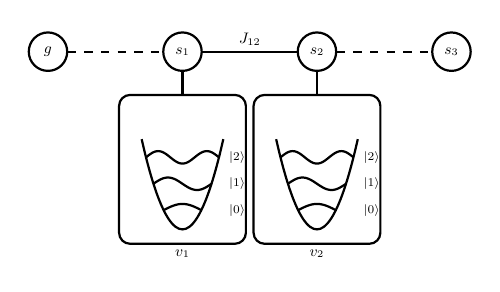
\begin{tikzpicture}[>=Stealth, site/.style={circle, draw, thick, minimum size=8mm, font=\small},
                          every node/.style={font=\small}, scale=0.61, transform shape]
        \node[site] (g)  at (0,0)   {$g$};
        \node[site] (s1) at (2.8,0) {$s_1$};
        \node[site] (s2) at (5.6,0) {$s_2$};
        \node[site] (s3) at (8.4,0) {$s_3$};
        \draw[dashed, thick] (g) -- (s1);
        \draw[thick] (s1) -- node[above] {$J_{12}$} (s2);
        \draw[dashed, thick] (s2) -- (s3);
        \foreach \x/\lab in {2.8/1, 5.6/2} {
          \draw[thick] (\x,-0.4) -- (\x,-0.9);
          \draw[rounded corners, thick] (\x-1.32,-0.9) rectangle (\x+1.32,-4.0);
          \draw[thick, domain=-0.85:0.85, smooth, variable=\t] plot ({\x+\t}, {-3.7+2.6*\t*\t});
          \foreach \n/\y in {0/-3.3, 1/-2.75, 2/-2.2} {
            \pgfmathsetmacro{\w}{sqrt((\y+3.7)/2.6)}
            \draw[thick, domain=-\w:\w, smooth, samples=50, variable=\u]
              plot ({\x+\u}, {\y+0.13*sin(deg((\n+1)*pi*(\u+\w)/(2*\w)))});
            \node[anchor=west, font=\scriptsize, inner sep=1pt] at (\x+0.93,\y) {$|\n\rangle$};
          }
          \node[below] at (\x,-4.0) {$v_\lab$};
        }
      \end{tikzpicture}
    \end{column}
    \begin{column}{0.57\textwidth}
      \begin{itemize}\setlength\itemsep{0.5em}
        \item One underdamped mode on each coupled site:
          \[ H=H_e+\sum_i\hbar\omega_m\,a_i^\dagger a_i+H_I \]
          \[ H_I=\sum_i \hbar g\,|s_i\rangle\langle s_i|\,(a_i+a_i^\dagger) \]
        \item Each mode is damped by its own thermal bath:
          \[ \gamma_M\sum_i\Big[(\bar n_M+1)\,\mathcal D[a_i]+\bar n_M\,\mathcal D[a_i^\dagger]\Big](\rho) \]
        \item Resonance: $\hbar\omega_m\approx\Delta E_{12}=200~\mathrm{cm^{-1}}$
        \item Coherent exchange $|\epsilon_1;n\rangle\leftrightarrow|\epsilon_2;n{+}1\rangle$
      \end{itemize}
    \end{column}
  \end{columns}
\end{frame}

% ---------------------------------------------------------------- 6
\begin{frame}{Mechanism of the enhancement}
  \centering
  % sizes chosen so that the plot frames of the two figures have the same top and bottom
  % (dressed states: frame rows 73.5-1035 of 1140 px; power panel: rows 69-814.5 of 960 px, top 62 px trimmed)
  \begin{tikzpicture}
    \node[anchor=south west, inner sep=0] (d) at (0,0)
      {\includegraphics[width=0.5867\textwidth]{discussion/dressed_states_benchmark.png}};
    \node[anchor=south west, inner sep=0] (img) at (0.6017\textwidth,-0.02126\textwidth)
      {\includegraphics[width=0.3783\textwidth,trim={1140 0 0 62},clip]{vibronic/iv_pv_vibronic.png}};
    \node[anchor=south west, draw=gray!60, fill=white, inner sep=2pt, align=left, font=\tiny,
          xshift=0.0832\textwidth, yshift=0.0656\textwidth] at (img.south west)
      {\textcolor{black}{\rule[0.4ex]{1.2em}{1pt}}\ Electronic model\\
       \textcolor{tblue}{\rule[0.4ex]{1.2em}{1pt}}\ Vibronic model};
  \end{tikzpicture}

  \vspace{0.8em}
  {\small Coupling mixes $|\epsilon_1;n\rangle$ and $|\epsilon_2;n{+}1\rangle$: mode damping (purple) adds a second path $\epsilon_1\to\epsilon_2$}

  \vspace{0.8em}
  Enhancement:\quad $\displaystyle\Delta P=\frac{P^\ast_{\mathrm{vib}}}{P^\ast_{\mathrm{el}}}-1=9.3\%$, as in Killoran \textit{et al.}
\end{frame}

% ---------------------------------------------------------------- 7
\begin{frame}{Research question and numerical cost}
  \begin{itemize}\setlength\itemsep{0.9em}
    \item A real environment has many modes, at different frequencies
    \item How does the enhancement change with more modes, or with modes off resonance?
    \item Direct solution: Liouville space of dimension $\big(d_e\,N_v^{M}\big)^2$
      \begin{center}
        \begin{tabular}{lcc}
          modes $M$ & 2 & 4 \\ \hline
          dimension & $2\times10^4$ & $3\times10^7$
        \end{tabular}
      \end{center}
    \item The cost grows exponentially with the number of modes, hence the use of DAMPF (Somoza \textit{et al.} 2019)
  \end{itemize}
\end{frame}

% ---------------------------------------------------------------- 8
\begin{frame}{Dissipation-assisted matrix product factorization}
  \begin{columns}[c]
    \begin{column}{0.5\textwidth}
      \centering
      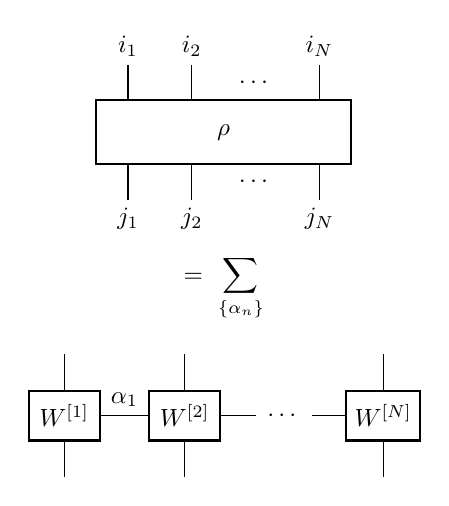
\begin{tikzpicture}[site/.style={draw, thick, minimum width=1.0cm, minimum height=0.7cm}, scale=0.9, transform shape]
        \node[draw, thick, minimum width=3.6cm, minimum height=0.9cm] (rho) at (0,2.3) {$\rho$};
        \draw (-1.35,2.75) -- ++(0,0.5) node[above] {$i_1$};
        \draw (-0.45,2.75) -- ++(0,0.5) node[above] {$i_2$};
        \node at (0.45,3.0) {$\cdots$};
        \draw (1.35,2.75) -- ++(0,0.5) node[above] {$i_N$};
        \draw (-1.35,1.85) -- ++(0,-0.5) node[below] {$j_1$};
        \draw (-0.45,1.85) -- ++(0,-0.5) node[below] {$j_2$};
        \node at (0.45,1.6) {$\cdots$};
        \draw (1.35,1.85) -- ++(0,-0.5) node[below] {$j_N$};
        \node at (0,0.1) {$=\ \displaystyle\sum_{\{\alpha_n\}}$};
        \begin{scope}[yshift=-1.7cm, xshift=-2.25cm]
          \node[site] (w1) at (0,0) {$W^{[1]}$};
          \node[site] (w2) at (1.7,0) {$W^{[2]}$};
          \node at (3.1,0) {$\cdots$};
          \node[site] (wn) at (4.5,0) {$W^{[N]}$};
          \draw (w1) -- (w2) node[midway, above] {$\alpha_1$};
          \draw (w2) -- (2.7,0);
          \draw (3.5,0) -- (wn);
          \draw (w1.north) -- ++(0,0.5); \draw (w1.south) -- ++(0,-0.5);
          \draw (w2.north) -- ++(0,0.5); \draw (w2.south) -- ++(0,-0.5);
          \draw (wn.north) -- ++(0,0.5); \draw (wn.south) -- ++(0,-0.5);
        \end{scope}
      \end{tikzpicture}
    \end{column}
    \begin{column}{0.48\textwidth}
      \begin{itemize}\setlength\itemsep{0.7em}
        \item Matrix product operator: one tensor per mode, linked by bond indices $\alpha_n$
        \item The bond dimension $\chi$ sets how much correlation between the modes is kept
        \item At fixed $\chi$ the cost grows linearly with the number of modes
        \item Damping drives each mode towards a thermal product state and limits the correlations: here $\chi_{\max}=8$
      \end{itemize}
    \end{column}
  \end{columns}
\end{frame}

% ---------------------------------------------------------------- 9
\begin{frame}{Implementation}
  \[ \rho=\sum_{m,n}|m\rangle\langle n|\otimes\hat O_{m,n},
     \qquad
     e^{\Delta t\,\mathcal L}\approx e^{\Delta t\,\mathcal L_{\mathrm{local}}}\,e^{\Delta t\,\mathcal L_{\mathrm{mix}}} \]
  \centering
  {\small\color{tgrey} electronic index outside the network, one MPO per block $\hat O_{m,n}$}

  \vspace{1.2em}
  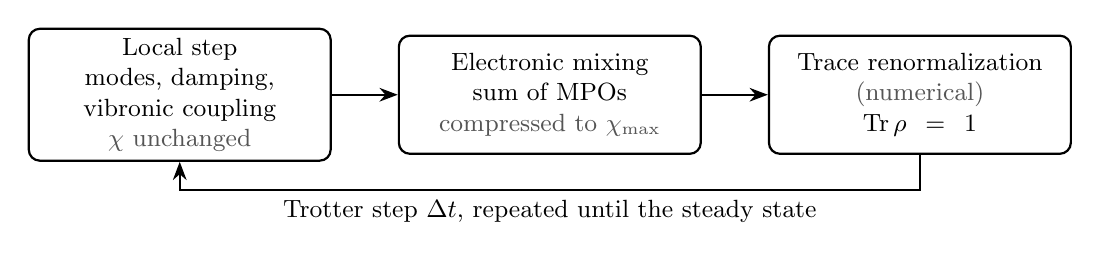
\begin{tikzpicture}[>=Stealth, box/.style={draw, thick, rounded corners, align=center, minimum height=1.5cm, text width=3.6cm, font=\small}]
    \node[box] (a) at (0,0) {Local step\\ modes, damping,\\ vibronic coupling\\ \textcolor{tgrey}{$\chi$ unchanged}};
    \node[box] (b) at (4.7,0) {Electronic mixing\\ sum of MPOs\\ \textcolor{tgrey}{compressed to $\chi_{\max}$}};
    \node[box] (c) at (9.4,0) {Trace renormalization\\ \textcolor{tgrey}{(numerical)}\\ $\mathrm{Tr}\,\rho=1$};
    \draw[->, thick] (a) -- (b);
    \draw[->, thick] (b) -- (c);
    \draw[->, thick] (c.south) -- ++(0,-0.45) -| node[pos=0.25, below, font=\small] {Trotter step $\Delta t$, repeated until the steady state} (a.south);
  \end{tikzpicture}

  \vspace{1.2em}
  Observables averaged over the steady-state plateau
\end{frame}

% ---------------------------------------------------------------- 10
\begin{frame}{Validation against the direct solution}
  \begin{columns}[c]
    \begin{column}{0.56\textwidth}
      \centering
      \includegraphics[height=0.76\textheight]{dampf/iv_curve_comparison_panel.png}
    \end{column}
    \begin{column}{0.42\textwidth}
      \begin{itemize}\setlength\itemsep{0.8em}
        \item Benchmark: one mode on $s_1$ and $s_2$, same truncation $N_v=6$
        \item Output power within 0.1\% near the maximum
        \item (d) Trace distance
          \[ D=\tfrac12\,\mathrm{Tr}\,\big|\rho_{\mathrm{DAMPF}}-\rho_{\mathrm{direct}}\big| \]
          $D\approx0.02$--$0.03$, an upper bound on the error of any observable
      \end{itemize}
    \end{column}
  \end{columns}
\end{frame}

% ---------------------------------------------------------------- 11
\begin{frame}{Additional modes}
  \begin{columns}[c]
    \begin{column}{0.47\textwidth}
      \centering
      \includegraphics[width=\textwidth]{confronti/power_maxwindow_configs.png}
    \end{column}
    \begin{column}{0.51\textwidth}
      \[ H_I=H_{CM}+H_{RD} \]
      \[ H_{RD}=\tfrac{\hbar g}{\sqrt2}\big(|\epsilon_1\rangle\langle\epsilon_2|+\mathrm{h.c.}\big)\big(a_{RD}+a_{RD}^\dagger\big) \]
      \[ a_{RD}=\tfrac{1}{\sqrt2}(a_1-a_2) \]
      \begin{itemize}\setlength\itemsep{0.6em}
        \item Only the relative displacement couples $\epsilon_1$ and $\epsilon_2$
        \item The center of mass, like a mode on $s_3$, couples to projectors that commute with $H_e$
        \item Two identical modes per site are one mode with coupling $\sqrt2\,g$: $+3\%$
      \end{itemize}
    \end{column}
  \end{columns}
\end{frame}

% ---------------------------------------------------------------- 12
\begin{frame}{Dependence on the mode frequency}
  \begin{columns}[c]
    \begin{column}{0.56\textwidth}
      \centering
      \includegraphics[width=\textwidth]{omega_gammaL_scan/enhancement_vs_omega_fixedg_fixedlambda.png}
    \end{column}
    \begin{column}{0.42\textwidth}
      \begin{itemize}\setlength\itemsep{0.8em}
        \item Fixed $g$: optimum close to resonance
        \item Fixed reorganization energy $\lambda=\hbar g^2/\omega$: optimum well above resonance, soft modes give the smallest enhancement
        \item At equal $\omega$, same thermal occupation in the two scans: the difference comes from how the coupling scales with $\omega$
      \end{itemize}
    \end{column}
  \end{columns}
\end{frame}

% ---------------------------------------------------------------- 13
\begin{frame}{A second mode on each site}
  \begin{columns}[c]
    \begin{column}{0.56\textwidth}
      \centering
      \includegraphics[width=\textwidth]{s1x2_s2x2_omega2_scan_rescaled/Pmax_vs_omega2_rescaled_vs_unscaled.png}
    \end{column}
    \begin{column}{0.42\textwidth}
      \begin{itemize}\setlength\itemsep{0.8em}
        \item One resonant mode and one at frequency $\omega_2$, on $s_1$ and $s_2$
        \item Fixed $\lambda$: a soft second mode lowers $P^\ast$ below the benchmark, a stiff one raises it
        \item Optimum at $\omega_2\approx350$--$400~\mathrm{cm^{-1}}$ in both conventions
        \item Same ordering with a cold or more strongly damped second mode
      \end{itemize}
    \end{column}
  \end{columns}
\end{frame}

% ---------------------------------------------------------------- 14
\begin{frame}{Sharing of the reorganization energy at fixed $\lambda$}
  \centering
  \includegraphics[width=0.86\textwidth]{discussion/coupling_share_fixed_lambda.png}
  \[ \lambda_{\mathrm{res}}=\lambda_0\,\frac{\omega_2}{\omega_2+\omega_m},\qquad
     \lambda_2=\lambda_0\,\frac{\omega_m}{\omega_2+\omega_m} \]
\end{frame}

% ---------------------------------------------------------------- 15
% Panels (a) and (c) of thesis figure 8.3 (left column), cropped
\begin{frame}{Non-additivity of the two modes}
  \centering
  \vspace*{\fill}
  \includegraphics[width=0.48\textwidth,trim={0 970 1142 0},clip]{discussion/redundancy_vs_omega2.png}\hspace{0.02\textwidth}%
  \includegraphics[width=0.48\textwidth,trim={0 45 1142 925},clip]{discussion/redundancy_vs_omega2.png}
  \vspace*{\fill}
\end{frame}

% ---------------------------------------------------------------- 16
\begin{frame}{Conclusions and outlook}
  \begin{itemize}\setlength\itemsep{0.6em}
    \item DAMPF implemented for the vibronic heat engine and validated against the direct solution (0.1\% on the power)
    \item Only the modes acting on the $\epsilon_1$--$\epsilon_2$ transition increase the power, and two such modes are partly redundant
    \item The best second mode lies well above resonance, as a trade-off between its own effect and its redundancy with the resonant mode
    \item The enhancement depends on how the vibronic coupling is distributed in frequency, as well as on its total strength
  \end{itemize}
  \vspace{0.6em}
  {\color{tblue}\textbf{Outlook}}
  \begin{itemize}\setlength\itemsep{0.4em}
    \item Explicit modes from a realistic spectral density (pseudomodes)
    \item Microscopic dissipative rates; non-Markovian residual bath
    \item Larger networks, where the tensor-network approach is most useful
  \end{itemize}
\end{frame}

% ================================================================ BACKUP
\appendix
\begin{frame}[plain]
  \centering\vfill{\Large\color{tblue}Backup slides}\vfill
\end{frame}

\begin{frame}{Local Lindblad dissipators}
  \begin{itemize}\setlength\itemsep{0.8em}
    \item Each dissipator acts on its own subsystem (excitons, or one mode), although the eigenstates of $H$ mix them
    \item Valid for Jaynes--Cummings-type systems if the transition frequencies are much larger than the dissipative rates and the bath spectrum is flat around them (Scala \textit{et al.} 2007)
    \item Here $\Gamma_C=8.07$ and $\gamma_M=5.3~\mathrm{cm^{-1}}$, on $200~\mathrm{cm^{-1}}$ splittings; the hot reservoir acts on a $\sim10^4~\mathrm{cm^{-1}}$ gap
    \item Same choice as Killoran \textit{et al.}: phenomenological rates, fixed by the bare energies
  \end{itemize}
\end{frame}

\begin{frame}{Markovian background and pseudomodes}
  \begin{itemize}\setlength\itemsep{0.8em}
    \item Explicit damped modes reproduce a structured bath correlation function
      \[ C(t)\approx\sum_k p_k\,e^{-i\Omega_k t-\gamma_k|t|/2} \]
    \item Pseudomode mapping: a non-Markovian bath becomes an enlarged, exactly Markovian problem (Tamascelli \textit{et al.} 2018)
    \item In this thesis the modes are taken from the Killoran model, not fitted, and the rest of the environment is memoryless
    \item This is the structure DAMPF is built for: explicit modes with local damping
  \end{itemize}
\end{frame}

\begin{frame}{Trace distance}
  \[ D(\rho,\sigma)=\tfrac12\,\|\rho-\sigma\|_1 \;\geq\; \frac{|\mathrm{Tr}[A(\rho-\sigma)]|}{2\|A\|} \]
  \begin{itemize}\setlength\itemsep{0.8em}
    \item Bounds the difference of every observable, over the full vibronic state
    \item Benchmark: $D\approx0.02$--$0.03$ over the whole $\Gamma_L$ range
    \item Current and power agree much better than this bound: the residual error is in the part of the state that does not enter the transport
  \end{itemize}
\end{frame}

\begin{frame}{Convergence in $\chi$}
  \begin{itemize}\setlength\itemsep{0.8em}
    \item The power grows monotonically with $\chi_{\max}$: a small $\chi$ cuts the vibronic correlations responsible for the enhancement
    \item Benchmark: $\chi_{\max}=6\to8$ changes $P$ by $0.2\%$
    \item Four modes: $8\to10$ changes $P$ by $0.1$--$0.3\%$, so differences below about $0.5\%$ are not resolved
    \item Two identical modes per site are equivalent to one mode with $\sqrt2\,g$: independent check of the four-mode runs
  \end{itemize}
\end{frame}

\begin{frame}{Thermal occupation and damping of the second mode}
  \begin{itemize}\setlength\itemsep{0.8em}
    \item Runs at $\omega_2=100,350,500~\mathrm{cm^{-1}}$, three load rates, with the second mode
      \begin{itemize}
        \item at zero temperature
        \item with doubled damping
      \end{itemize}
    \item Doubled damping: changes of a few tenths of a percent, same ordering
    \item Cold second mode: never more favorable; the largest decrease is for the softest mode
    \item Neither the occupation nor the damping of the second mode determines the optimum
  \end{itemize}
\end{frame}

\begin{frame}{Polaron shift and reorganization energy}
  \begin{itemize}\setlength\itemsep{0.8em}
    \item The coupling lowers the site energies by $\lambda=\hbar g^2/\omega$ (no counterterm in the model)
    \item Equal shift on $s_1$ and $s_2$, rates fixed by the bare energies: no effect on the steady state
    \item Checked directly: with and without counterterm, the same $9.3\%$
    \item The dependence on $\lambda$ found in the scans is therefore dynamical
  \end{itemize}
\end{frame}

\begin{frame}{CM/RD reduction and DAMPF}
  \begin{itemize}\setlength\itemsep{0.8em}
    \item The CM/RD reduction relies on the symmetry of this model: identical modes on $s_1$ and $s_2$, $E_1=E_2$, $J_{13}=J_{23}=0$
    \item It does not apply with different modes on the two sites, couplings to $s_3$, larger networks or many modes per site
  \end{itemize}
\end{frame}

\begin{frame}{Fock truncation $N_v=6$}
  \begin{itemize}\setlength\itemsep{0.8em}
    \item The steady-state population is concentrated in the lowest doublets: the mechanism involves the first few quanta
    \item In the $g=0$ limit, $N_v=6$ reproduces the electronic model to $10^{-10}$
    \item Same truncation in DAMPF and in the direct solution, so the comparison isolates the Trotter and $\chi$ errors
  \end{itemize}
\end{frame}

\end{document}
